\documentclass{article}

\usepackage{tikz}
\usepackage{pgfplots}
\usepackage{xcolor}
\pgfplotsset{compat=1.17}

\definecolor{myblue}{RGB}{54,106,146}
\definecolor{mygray}{RGB}{240,240,240}

\begin{document}

\begin{center}
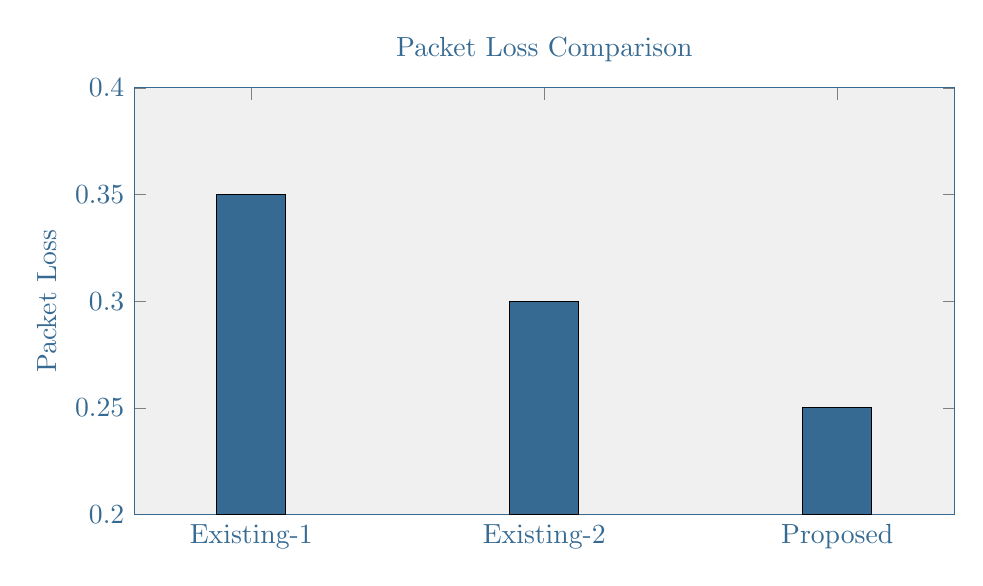
\begin{tikzpicture}
\begin{axis}[
    width=12cm,
    height=7cm,
    title={Packet Loss Comparison},
    title style={color=myblue},
    ylabel={Packet Loss},
    ylabel style={color=myblue},
    tick label style={color=myblue},
    axis line style={color=myblue},
    ymin=0.2,
    ymax=0.4,
    ytick={0.2,0.25,0.3,0.35,0.4},
    symbolic x coords={Existing-1, Existing-2, Proposed},
    xtick=data,
    bar width=25pt,
    enlarge x limits=0.2,
    axis background/.style={fill=mygray}
]

\addplot[ybar, fill=myblue] coordinates {
    (Existing-1, 0.35)
    (Existing-2, 0.30)
    (Proposed, 0.25)
};

\end{axis}
\end{tikzpicture}
\end{center}

\end{document}